\documentclass[12pt,a4paper]{article}
\usepackage[top=25.4mm, bottom=25.4mm, left=19.1mm, right=19.1mm]{geometry}


\usepackage[latin2]{inputenc}
\usepackage{graphicx}
\graphicspath{ {./images/} }
\usepackage{ulem}
\usepackage{amsmath}
\usepackage[document]{ragged2e}

\setlength{\parindent}{4em}
\setlength{\parskip}{1em}
\usepackage{hyperref}

\usepackage{fancyhdr}
\pagestyle{fancy}
\fancyhf{}
\fancyhead[LO]{\textbf{\small IoT and Smart Analytics}\\
\text{\small A Program by IIITH and TalentSprint}}

\usepackage{xcolor}
\usepackage{lipsum}

\rhead{\begin{picture}(0,0) \put(-250,-2){
\includegraphics[width=9cm]{EXP_06_Images/ts-iisc-logo-pr.png}} \end{picture}}
\cfoot{\thepage}


\begin{document}

\begin{center}

\textbf{\large \\EXPERIMENT 18}\\[6pt]
\text{ ESP32 WiFi Repeater  }
\end{center}

\textbf{\large LEARNING OBJECTIVES:}\\[3pt]
At the end of this experiment, participants will be able to:\vspace{-6mm}\begin{enumerate}
 \setlength\itemsep{-0.3em}
\item Understand how to implement a WiFi repeater using ESP32 \\
\end{enumerate}
\textbf{\large APPARATUS REQUIRED:}\\
\vspace{-3mm}
\begin{enumerate}
 \setlength\itemsep{-0.3em}
\item ESP32 Module\\
\item Micro USB cable\\
\end{enumerate}

\begin{justify}
\textbf{\large THEORY}\\[3pt]
\textbf{Introduction:} In this experiment, a standalone WiFi repeater would be implemented using an ESP32 board, extending the existing WiFi range. You can also use antennas to improve the range. One such example is shown in links: \href{https://www.espressif.com/en/news/esp32%E2%80%99s-wi-fi-range-extended-10-km-directional-antenna}{ESP32 WiFi Range Testing-10km}, and \href{https://www.youtube.com/watch?v=yCLb2eItDyE} {video} .

\noindent In above example the WiFi range is extended to 10km. Typically, a household WiFi router would provide a signal to not more than a few meters when considering the line of sight and lesser distance with obstacles in between. The device, when configured as a repeater, will help you to extend your existing WiFi network. A lot of smart home appliances will require WiFi connectivity to control all of them remotely. So we can set up an independent WiFi network with different SSID and Passwords for these devices. Another example, we can also use this device to provide independent internet connectivity to the guests because, unlike ESP8266 repeater, we can achieve a bandwidth of almost 15mbps, almost 3 times more. This means that browsing the internet and stream videos without interruption. A ESP32 WiFi repeater or expander works by receiving your existing WiFi signal, amplifying it, and then transmitting the enhanced signal.\par
\noindent There is no coding involved in converting the ESP32 board into a repeater, but we need two things:
\begin{enumerate}
 \setlength\itemsep{-0.3em}
\item \href{https://www.espressif.com/en/support/download/other-tools} {ESP Flash Download Tools}  (Download only the flash tool)\\
\item  \href{https://github.com/martin-ger/esp32_nat_router}{ESP WiFi Repeater firmware} (Download the entire repository)
\end{enumerate}
After downloading the above files, extract the zip folders and follow the procedures below.\\[14pt]
\noindent \textbf{\large PROCEDURE}\\[6pt]
\textbf{A)	Flash the firmware on ESP32 board:}
\vspace{-6mm}
\begin{enumerate}
\setlength\itemsep{-0.3em}
\item After extracting the files, open the flash tool as administrator. The window shown in fig.1 will appear.
\item In the window, select the chip type to be ESP32 and workmode to be developer.
\item After, this an interface, as shown in fig.2, will appear where you need to select the bootloader, esp32 nat router, and partition file.
\begin{center} 
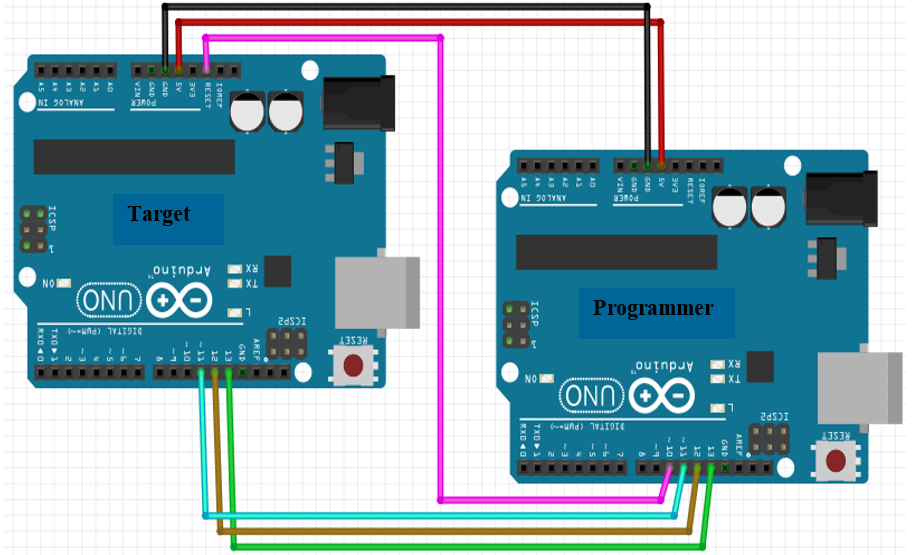
\includegraphics[scale=0.9]{EXP_18_Images/fig1.png}
\end{center}
\begin{center} {Figure 1. ESP32 Flash tool  }\end{center}
\begin{center} 
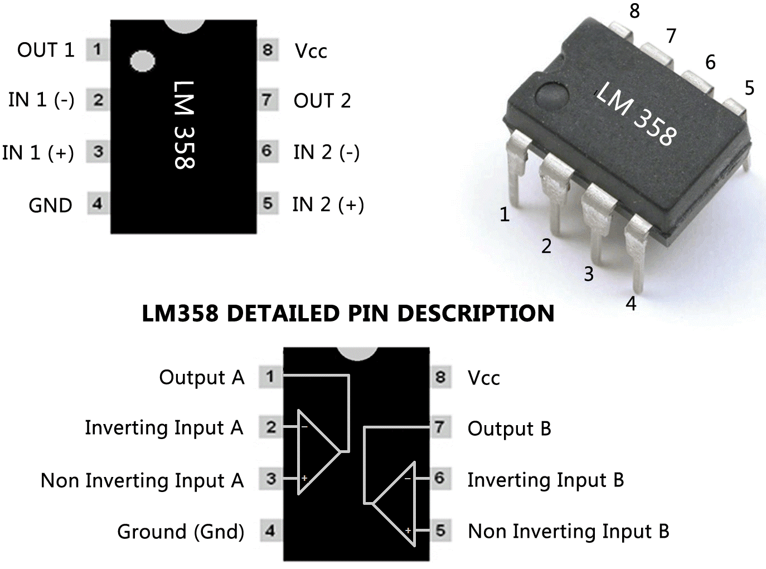
\includegraphics[scale=0.7]{EXP_18_Images/fig2.png}
\end{center}
\begin{center} {Figure 2. ESP32 Flash tool configuration }\end{center}

\noindent Firstly, click on the first row, and it will bring us to the file explorer. Then select the bootloader.bin file from the ESP firmware folder. When it is added, the row turns green.\\
$\rightarrow build  \rightarrow  bootloader \rightarrow bootloader.bin.$
\item Next, select the next row and choose the esp32\_nat\_router.bin file.\\
$\rightarrow build \rightarrow  bootloader \rightarrow esp32\_nat\_router.bin.$
\item Finally, select the partition file.\\
$\rightarrow build  \rightarrow bootloader \rightarrow pratitions\_example.bin.$
\item Now, specify the hexadecimal code indicating where the files are. For bootloader type write 0x1000, for esp32 nat router file write 0x10000, and for the partition file 0x8000.
\item Now tick all these three boxes and as you complete this also, the address box also changes to green.
\item The rest of these settings are at their default at where they are, as seen in fig.2. The SPI speed is 40MHz and SPI Mode is DIO.
\item Now to upload the firmware, the COM port of our ESP32 needs to be selected.
\item Note that You might have to press and hold the boot button on the board and press the start button to start flashing firmware depending on your board.
\item Now, the device MAC shows up in the same window, and then the green line starts to load and then you see the finish sign on the left. Now you can restart the ESP32 board.
\end{enumerate}

\begin{center} 
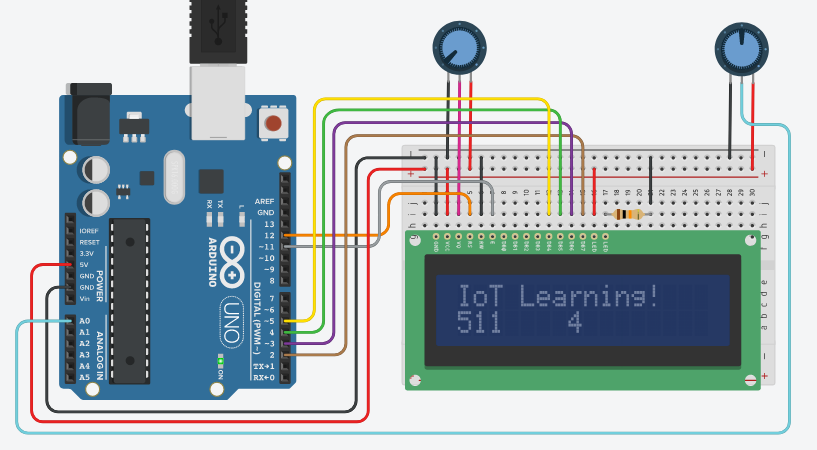
\includegraphics[scale=0.9]{EXP_18_Images/fig3.png}
\end{center}
\begin{center} {Figure 3. Flash tool after upload}\end{center}

\textbf{B)	Configuring WiFi Repeater:}
\vspace{-6mm}
\begin{enumerate}
\setlength\itemsep{-0.3em}
\item Now connect a mobile/computer to your ESP32 in order to configure it. After the first boot, the board provides an open WiFi with SSID ESP32\_NAT\_Router. Connect to this WiFi network. Then perform basic configuration via a simple web interface by going to the address http://192.168.4.1 
\item Now the page in fig.4 can be seen.

\begin{center} 
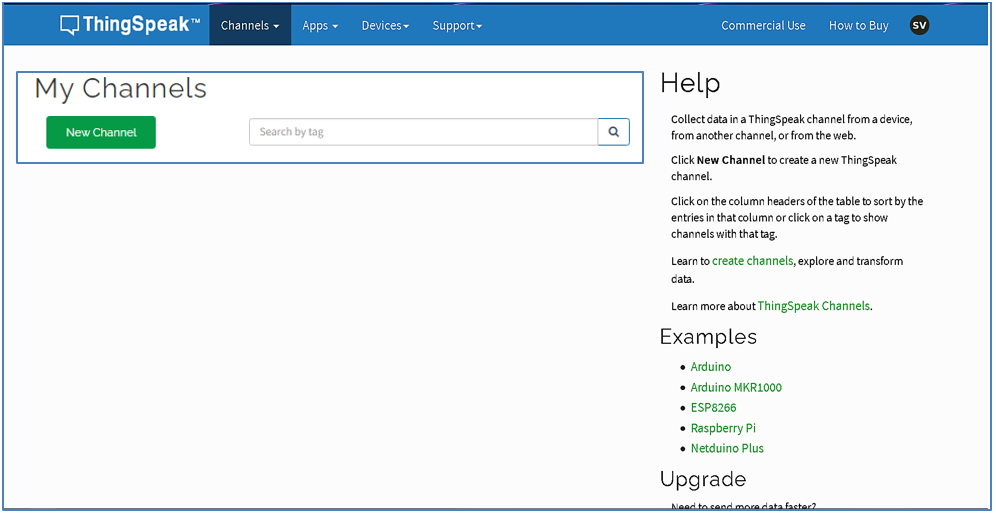
\includegraphics[scale=1]{EXP_18_Images/fig4.png}
\end{center}
\begin{center} {Figure 4. ESP32 NAT Router Configuration}\end{center}
\item Firstly, in the STA settings enter the credentials of the main WiFi network that needs to be extended. Leave the password field for open networks. Click on Connect. The board reboots and will connect to your WiFi router. You might have to connect to the ESP32\_NAT\_Router ssid again.
\item Reload the page. To change the AP Settings type the New SSID and Password and then click Set. The ESP reboots again. Now it can forward traffic over the newly configured Access Point.
\item You can give static IP settings if needed or else leave it empty to use DHCP.
\item Remember that these changes also affect the configuration interface, i.e. to do further configuration, enter the IP address of the new Access point configuration.
\end{enumerate}
\setlength{\parindent}{0eM}
\textbf{\large REFERENCE :}
\begin{enumerate} 
\setlength\itemsep{-0.3em}
\item \href{https://github.com/martin-ger/esp32_nat_router}{
ESP32 NAT Router}
\item \href{https://www.espressif.com/en/support/download/other-tools  } {ESP Flash Download Tools}
\end{enumerate}
\end{justify}
\end{document}